\section{Database}
To support the necessary information storage, a database is implemented in accordance with the ER diagram described in \secref{sec:ERdiagram}.
The implementation of the ER diagram leads to the database schema that can be seen in \figref{fig:Database-tables}, however, there is more than just what the ER diagram describes.
In this figure, the connections between the tables represents foreign key constraints.

\begin{figure}[h]
	\centering
	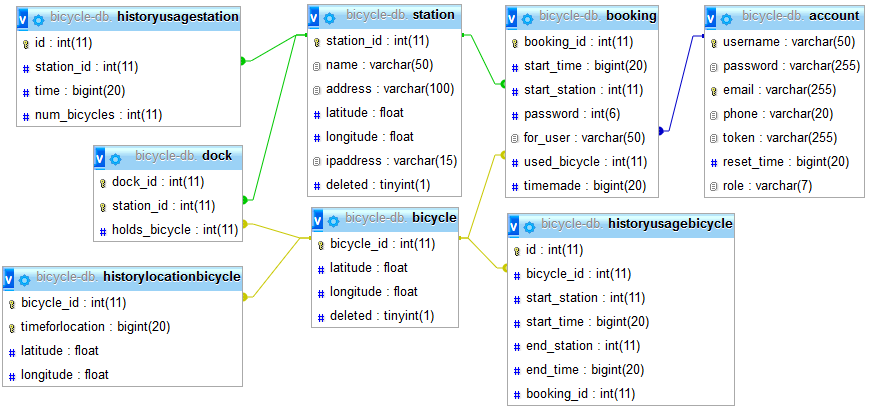
\includegraphics[scale=0.6]{Database/DBtables}
	\caption{Database tables}\label{fig:Database-tables}
\end{figure}

The additional tables(historyusagestation, historyusagebicycle and historylocationbicycle) are added to store the information needed for the features described in \secref{sec:designAdminTools} and which implementation is discussed in \secref{sec:impAdminTools}.
The three additional tables serves as a log, in order to store information about usage of the system, to be used by the administration part of the system to analyse on the usage of the system.

In the translation from the ER diagram to the schema presented, the relations between the various entities could in all cases be represented as an attribute on one of the involved entities.
This attribute is a foreign key.
This was all that was needed to convert the ER diagram into the database schema, however, with the introduction of the admin features and their associated data tables, more was needed.

When the admin features was added into the database, in addition to adding three new tables to contain their information.
The admin features also required addition of additional attributes to some of the already existing tables, an example of this being \textit{role} attribute on the account table, used to distinguish regular users from the ones with admin privileges.

\fxwarning{der skal skrives til: ekstra attributes, naevn mysql}